\documentclass[12pt, oneside]{article}   	
\usepackage{geometry}                		
\geometry{a4paper}                   		
%\usepackage[spanish, es-noindentfirst]{babel}
%\selectlanguage{spanish}
%\usepackage[utf8]{inputenc}               		
    		
\usepackage{graphicx}	
\usepackage{caption}
\usepackage{subcaption}		
\usepackage{float}	
										
\usepackage{amssymb}
\usepackage{amsmath}
\usepackage{authblk}
\usepackage{bm}
%\usepackage[lite]{mtpro2}

\usepackage{booktabs}

\pagenumbering{gobble}
\usepackage{verbatim}
\immediate\write18{texcount -tex -sum  \jobname.tex > \jobname.wordcount.tex}

% Keywords command
\providecommand{\keywords}[1]
{
  \small	
  \textbf{\textit{Keywords:}} #1
}


\newcommand{\bx}{\mathbf{x}}
\newcommand{\bu}{\mathbf{u}}
\newcommand{\bz}{\mathbf{z}}
\newcommand{\bA}{\mathbf{A}}
\newcommand{\bX}{\mathbf{X}}
\newcommand{\bY}{\mathbf{Y}}
\newcommand{\bV}{\mathbf{V}}
\newcommand{\bbeta}{\bm{\beta}}
\newcommand{\myeta}{\bm{\eta}}
\newcommand{\indep}{\rotatebox[origin=c]{90}{$\models$}}

\title{Estimation of average treatment effect for ACIC Data Challenge}
\author[]{Wanwan Xu}
\affil[]{Univeristy of Connecticut, Department of Statistics}
\renewcommand\Authands{, }
\date{}							

\begin{document}
\maketitle

\begin{abstract}
This is a data-driven project based on ACIC 2019 data challenge, the main objective is to estimate the population average treatment effect (ATE). The performance of regression estimator, inverse propensity weighted estimator, augmented inverse propensity weighted estimator and calibration estimator is compared on test datasets as well as some theoretical properties. The final result for all 3,000 sets of training data is also presented. 
\end{abstract}
\keywords{average treatment effect, counterfactual, causal inference}

\section{Introduction}
Treatment effect has always been of interest, as it quantitatively  show the causal effect of a binary variable on an outcome variable. This 0-1 variable, also called treatment, is now used much more generally than a medical procedure or experimental drug. In economics, the causal effect of a subsidized training program \cite{Ashenfelter1978} is widely analyzed, so are the effects of active labor market programs such as job search assistance or classroom teaching program \cite{LaLonde1986}. Since treatment effect is defined as the difference between two treatment groups, while in reality, one unit or one observation is only related to one of the treatment assignment, it's impossible to measure causal effects at the individual level, therefore we focus on the expectation, i.e. average treatment effect(ATE). In experimental study, randomized trial is a gold standard to identify average treatment effects. But in order to achieve randomization, the balance distributions of subject characteristics across groups is required, so that groups are similar except for the treatments, it may be infeasible, or even unethical, to conduct in practice. On the other hand, observational studies are common in economy, social science, and public health, where the participation of intervention is only observed rather than controlled by designers. A typical concern for inferring causality in an observational study is confounding, treatment exposure may e associated with covariates that are also associated with potential response. For example, experiment individual characteristics such as demographic factors can be related to both the treatment selection and the outcome of interest. 

In order to perform unbiased comparison despite the confounding factors, the inferences with causal interpretation need to be adjusted. There are three broad classes of strategies, outcome regression, propensity score estimation and nonparametric estimation. For outcome regression, the model of outcome given covariates need to be specified, then it can be used for predicting unobserved potential outcomes and estimating ATE \cite{Oaxaca1973}. It follows similar procedure of calculating counter factuals. For propensity score estimation, Rosenbaum and Rubin \cite{Rosenbaum1983} proposed several properties that facilitate causal inferences. A popular method for estimating the causal difference of two treatment means is to stratifying individuals based on estimated propensity scores, then use the average of within stratum effects as ATE \cite{Rosenbaum1984}. An alternative approach is to construct weights for individual observations via using estimated propensity scores. individual observations \cite{Robins2000}. Above two classes require specification of propensity score model or outcome model or both, some nonparametric estimators are then developed to provide valid inference in large samples without relying on parametric assumptions in the intermediate steps of estimation \cite{Chen2008}. Chan  \cite{Chan2016} applied the class of survey calibration estimators on the estimation of average treatment effects, the authors also showed that a globally efficient estimator can be adapted from it. 

This report focuses on applying several estimation methods described above to ACIC data challage low dimension track datasets. The report is organized as follows. In Section \ref{sec:data}, we introduce the data structure and explanation. The methods applied is briefly introduced in Section \ref{sec:method}, the comparison based on test dataset is presented in Section \ref{sec:result} as well as the results for training dataset. Some final remarks and future directions are given in Section \ref{sec:disc}.

\section{Dataset}\label{sec:data}
\subsection{Introduction}
Two tracks of data (low dimension and high dimension) are included in the ACIC data challenge, each track have 3200 csv files drawn from 32 unique data generating processes (DPG). In this report, we focus only on low dimensional track. Within each csv file, there are:
\begin{itemize}
\setlength\itemsep{-0.5em}
\item response variable $\bY=\{Y_1,Y_2,\ldots,Y_n\}$, half are continuous while the other half is discrete;
\item binary treatment indicator $\bA=\{A_1,A_2,\ldots,A_n\}$;
\item pre-treatment covariates $\bV=\{V_1,\ldots,V_p\}$, which includes the mixture of continuous, binary, and categorical variables.
\end{itemize}

In order to understand the data structure better, we made an example of the first dataset into clinical trial framework. Suppose a trial is designed to analyze whether a specific drug can lower blood pressure or not. Data from $n=668$ patients are collected, some of them are assigned to take the drug ($A_i=1$) and others took placebo ($A_i=0$). Their pre-treatment vital is recorded as well. For example race and gender are saved as catogorical, certain disease history is saved as binary, and patients' height, weight, temperature are saved as continuous. After the treatment, their blood pressure change is recorded in $\bY$. Each of the dataset can be explained by such similar "stories", the goal is to find an appropriate model that can perform good on all the datasets. 

Aside from the mixture of data type, number of covariates and number of observations may also be different for each worksheet as shown in Figure \ref{fig:pie}.

\begin{figure}[!htb]
\begin{subfigure}{.5\textwidth}
  \centering
  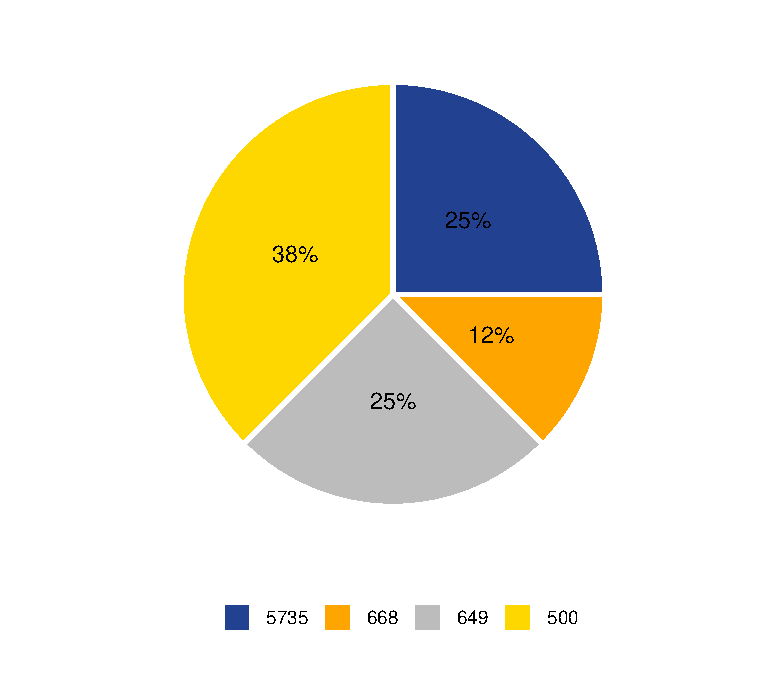
\includegraphics[width=1\linewidth]{../plot/obs_freq}
  \caption{number of observations}
\end{subfigure}%
\begin{subfigure}{.5\textwidth}
  \centering
  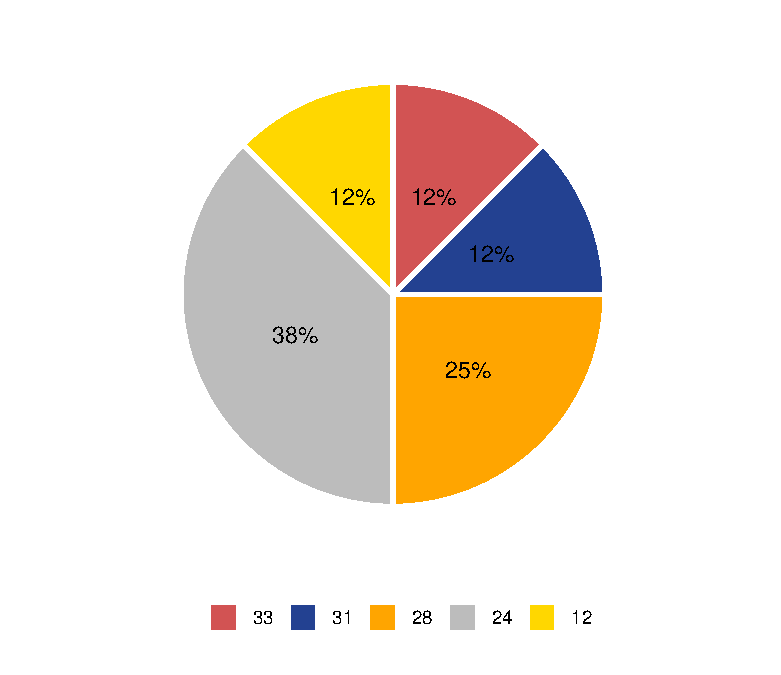
\includegraphics[width=1\linewidth]{../plot/var_freq}
  \caption{number of covaraibles}
\end{subfigure}
\caption{Frequency plot low track dataset}
\label{fig:pie}
\end{figure}

The description site of data challenge also provided some more information. For instance, there are no mediators among covariates, that is we only need to consider direct effect from covariates. Also, all the covaraites also include all the cofounders, we don't need to consider hidden variables. However, selection variables may still exists, given some of the covaraites may be related to the treatment factor $\bA$.

  
\subsection{Objectives}
The measure of estimation is the population average treatment effect (ATE) and 95\% confidence interval for each dataset. For individual $i \in \{1,2,\ldots,n\}$, denote $Y_{0i}$ as the outcome variable for individual $i$ if he/she is not treated, $y_{1i}$ as the value of the outcome variable for individual $i$ if he/she is treated. The treatment effect for individual $i$ is given by $Y_{1i}-Y_{0i}=\beta_i$. In the general case, there is no reason to expect this effect to be constant across individuals. The average treatment effects is given by 
$$\mbox{ATE}=E[Y_{1i}-Y_{0i}].$$
where the expectation is with respect to the distribution of covariates. However, in observational data, we can only observe one of the two for each individual, thus estimation techniques are needed. Under this circumstances, one of the $y_{0i},y_{1i}$ will be replaced by counterfactual output. Since the causal assumptions of consistency and strong ignorability are guaranteed, the target statistical estimand can be rewritten as:
$$\mbox{ATE}=E[E(\bY | \bA = 1, \bV) - E(\bY | \bA = 0, \bV)]$$

\subsection{Difficulties}
Apart from the complicated structure of the data and requirement for generality of applied model, there are a few more challenges for this specific objective.
\begin{itemize}
\setlength\itemsep{-0.5em}
\item Non-linearity of the response surface. Not only does the distribution of covaraites $\bV$ is unknown, the model may also be non-linear. 
\item Treatment effect heterogeneity. There may exist differences across subjects, going back to the clinical trail example, different patients may have different response level for the same treatment. 
\item Varying proportion of true confounders among the observed covariates. Even though we are provided with the fact that all the confounders are measured and included in the covariste set, the proportion or location of these confounders still remain unknown. 
\end{itemize}
    
\section{Method}\label{sec:method}
\subsection{Notation}
Following the notation of dataset, use $i \in \{1,2,\ldots,n\}$ to denote $i$th observation, $Y_i$ as observed outcome, $A_i\in \{0,1\}$ as treatment assignment, $\bV=\{V_1,V_2,\ldots,V_p\}$ as the set of covaraites, $Y_i(1)$ as potential outcome if $A_i=0$ and $Y_i(0)$ as potential outcome if $A_i=1$. Furthermore, we use $\pi(\bV)=P(\bA=1|\bV)$ to denote propensity score.

There are a few common assumptions for the methods discussed below: (1)all units $Y_i$ are random sampled; (2)the treatment value is stable such that potential outcomes $Y_i(1), Y_i(0)$ are completely determined and the observed outcome will be equal to the potential outcome corresponding to the assigned treatment: $Y_i=A_iY_i(1)+(1-A_i)Y_i(0)$; (3) strong ignorability $\{\bY(0),\bY(1)\} \indep \bA|\bV$; (4)plausible range of propensity score function $0<\pi(\bV)<1$.

\subsection{Regression Estimator (REG)}
Lots of traditional causal estimation relies on the formulation of a regression model for the outcome variable $\bY$. In other words, the focus is on the estimation of $E[\bY|\bA,\bV]$. Given ATE is defined with respect to the distribution of covariates, the empirical distribution will be an easy estimate of $F_{\bV}$. Thus the regression estimate can be written as:
\begin{equation}
\widehat{\mbox{ATE}}_{REG}=\frac{1}{n}\sum_{i=1}^n \{E(\bY | \bA = 1, V_i) - E(\bY | \bA = 0, V_i)\}
\end{equation}
where the conditional expectation functions can be estimated using any consistent estimator. Options include ordinary least squares, generalized linear models, generalized additive models (GAMs), local regression, kernel regression, etc \cite{Pearl2002}. 

Even though the regression estimator for ATE is easy to understand, the shortcoming is also obvious. It depend heavily on the estimation method and the choice of regression model, especially with high dimensional $\bV$, it may be difficult to estimate both regression functions over the full range of Z. It has been shown when the observed values of $\bV$ are not similar for the treatment and the control groups, then one of the conditional expectation functions will often be poorly estimated \cite{King2006}. However, in our dataset, this problem doesn't seem to appear, so the regression estimator is also included in the comparison.


\subsection{Inverse Propensity Weighted Estimator (IPW)}
Another widely applied method for estimating ATE relies on a model for treatment
assignment instead a regression model for the outcome. Suppose the true probability
of assigning treatment were known, this could be used to define propensity scores, and further be used for matching or weighting covariates. A well-known weighting estimator is the IPW estimator:
\begin{equation}
\widehat{\mbox{ATE}}_{IPW}=\frac{1}{n}\sum_{i=1}^n \left\{\frac{A_iY_i}{\hat{\pi}(\bV_i)}-\frac{(1-A_i)Y_i}{1-\hat{\pi}(\bV_i)}\right\}
\end{equation}
where $\hat{\pi}(\bV_i)$ is the estimated propensity score, that is the estimated conditional probability of treatment given $\bV_i$. As stated by Glynn in \cite{Imbens2004}, if the propensity score estimate is consistent, the IPW estimator is consistent as well. However, as can be seen in the formula, observations with $A_i=1$ and $\hat{\pi}(\bV_i)$ close to 0 may contribute extremely to the estimate, similarly to the observations with the untreated group of $A_i=0$ and $\hat{\pi}(\bV_i)$ close to 1. In some cases, these extreme contributions can produce implausible estimate of ATE (greater than 1). Therefore here we apply one of the improvements to the basic IPW estimator proposed by \cite{Imbens2004}. The authors re-normalize the weights so that they sum to one:
\begin{equation}
\widehat{\mbox{ATE}}_{IPW^*}=\left\{\sum_{i=1}^n \frac{A_i}{\hat{\pi}(\bV_i)}\right\}^{-1}\sum_{i=1}^n \frac{A_iY_i}{\hat{\pi}(\bV_i)}-\left\{\sum_{i=1}^n \frac{1-A_i}{1-\hat{\pi}(\bV_i)}\right\}^{-1}\sum_{i=1}^n\frac{(1-A_i)Y_i}{1-\hat{\pi}(\bV_i)}
\end{equation}


\subsection{Augmented Inverse Propensity Weighted \\Estimator (AIPW)}
Based on the previous work of IPW estimation, one improvement including fully utilizing the information in the conditioning set $\bV$ is AIPW \cite{Glynn2010}. Aside from the information about treatment assigning probability, $\bV$ also carry the predictive information about the response variable $\bY$:
\begin{equation}
\begin{split}
\widehat{\mbox{ATE}}_{AIPW} = \frac{1}{n}\sum_{i=1}^n & \bigg\{\left[ \frac{A_iY_i}{\hat{\pi}(\bV_i)}-\frac{(1-A_i)Y_i}{1-\hat{\pi}(\bV_i)}\right] - \frac{(A_i-\hat{\pi}(\bV_i))}{\hat{\pi}(\bV_i)(1-\hat{\pi}(\bV_i))} \\
& [(1-\hat{\pi}(\bV_i))\hat{E}(Y_i|A_i=1,\bV_i)+\hat{\pi}(\bV_i)\hat{E}(Y_i|A_i=0,\bV_i)]\bigg\}
\end{split}
\end{equation}

Similar to IPW estimand, AIPW also needs to specify a binary regression model for the propensity score, and specify a regression model for the outcome variable. However, as summarized by the authors, AIPW has so called ``double robustness'' property. Simply speaking, the estimator remains consistent for the ATE if either the propensity score model or the outcome regression is misspecified but the other is properly specified. AIPW estimator are also shown to be asymptotically normally distributed and valid large-sample standard errors can be derived through the theory of M-estimation. One advantage of AIPW method in our data application is it provides multiple ways of calculating sample variance, including an empirical sandwich estimator proposed by Lunceford \cite{Luncefird2004}, alternative large-sample results as well as the bootstrap. 

\subsection{Calibration Estimator (CAL)}
Previous few estimate methods both require estimation of a propensity score function, and an outcome regression function, IPW and AIPW is globally semiparametric efficient when a sieve maximum likelihood propensity score estimator is used. Chan \cite{Chan2016} proposed a wide class calibration weights to attain the moments of observed covariates among the treated, the control, and the combined group. Furthermore, these empirical weights can be applied for globally efficient non-parametric inference of ATE. Chan and Yam reformulated the problem into optimization framework:
\begin{equation}
\begin{split}
\mbox{min} & \sum_{i=1}^nA_iD(np_i,1)\quad s.t.\quad \sum_{i=1}^nA_ip_iu_K(\bV_i)=\frac{1}{n}\sum_{i=1}^nu_K(\bV_i), \\
\mbox{min} & \sum_{i=1}^n(1-A_i)D(nq_i,1)\quad s.t.\quad \sum_{i=1}^n(1-A_i)q_iu_K(\bV_i)=\frac{1}{n}\sum_{i=1}^nu_K(\bV_i) 
\end{split}
\end{equation}
where $u_K$ is a $K(N)$-dimensional function of $\bV$, $D$ is chosen distance measure. The proposed empirical balancing estimator for ATE is:
\begin{equation}
\widehat{ATE}_{CAL} = \sum_{i=1}^n\{A_i\hat{p}_K(\bV_i)Y_i-(1-A_i)\hat{q}_K(\bV_i)Y_i\}
\end{equation}
where $\hat{p}_K,\hat{q}_K$ are the dual solutions for above equation. One thing worth noticing here is the usage of concave function $\rho(v)$ when solving the dual optimization problem. In \cite{Chan2016}, four different functions are used, including exponential tilting (ET) $\rho(v)=-e^{-v}$; empirical likelihood (EL) $\rho(v)=log(1+v)$; quardratic (Q) $\rho(v)=-(1-v^2)/2$ and inverse logistic (IL) $\rho(v)=v-e^{-v}$. In our data application, we apply the ET version, which is also shown to be the ``best'' selected by simulation part in the paper.

\section{Result}\label{sec:result}

\section{Discussion}\label{sec:disc}
%There are a few possible directions to try out:
%\begin{enumerate}
%\item choice of propensity function
%\item choice of smooth function
%\item fast implementation of bootstrap etc
%\item sampling and population ATE
%\item comparison between propensity and weight
%\end{enumerate}


%
% ---- Bibliography ----
%


\begin{thebibliography}{5}
\bibitem{Ashenfelter1978}
Ashenfelter, Orley. "Estimating the effect of training programs on earnings." The Review of Economics and Statistics (1978): 47-57.

\bibitem{Chambers1992}
Chambers, John M., and Trevor J. Hastie, eds. Statistical models in S. Vol. 251. Pacific Grove, CA: Wadsworth \& Brooks/Cole Advanced Books \& Software, 1992.

\bibitem{Chan2016}
Chan, Kwun Chuen Gary, Sheung Chi Phillip Yam, and Zheng Zhang. "Globally efficient non‐parametric inference of average treatment effects by empirical balancing calibration weighting." Journal of the Royal Statistical Society: Series B (Statistical Methodology) 78.3 (2016): 673-700.

\bibitem{Chen2008}
Chen, Xiaohong, Han Hong, and Alessandro Tarozzi. "Semiparametric efficiency in GMM models with auxiliary data." The Annals of Statistics 36.2 (2008): 808-843.

\bibitem{Glynn2010}
Glynn, Adam N., and Kevin M. Quinn. "An introduction to the augmented inverse propensity weighted estimator." Political analysis 18.1 (2010): 36-56.

\bibitem{Imbens2004}
Imbens, Guido W. "Nonparametric estimation of average treatment effects under exogeneity: A review." Review of Economics and statistics 86.1 (2004): 4-29.

\bibitem{King2006}
King, Gary, and Langche Zeng. "The dangers of extreme counterfactuals." Political Analysis 14.2 (2006): 131-159.

\bibitem{LaLonde1986}
LaLonde, Robert J. "Evaluating the econometric evaluations of training programs with experimental data." The American economic review (1986): 604-620.

\bibitem{Luncefird2004}
Lunceford, Jared K., and Marie Davidian. "Stratification and weighting via the propensity score in estimation of causal treatment effects: a comparative study." Statistics in medicine 23.19 (2004): 2937-2960.

\bibitem{Oaxaca1973}
Oaxaca, Ronald. "Male-female wage differentials in urban labor markets." International economic review (1973): 693-709.

\bibitem{Pearl2002}
Pearl, Judea. "Causality: models, reasoning, and inference." IIE Transactions 34.6 (2002): 583-589.

\bibitem{Robins2000}
Robins, James M., Miguel Angel Hernan, and Babette Brumback. "Marginal structural models and causal inference in epidemiology." (2000): 550-560.

\bibitem{Rosenbaum1983}
Rosenbaum, Paul R., and Donald B. Rubin. "The central role of the propensity score in observational studies for causal effects." Biometrika 70.1 (1983): 41-55.
 
\bibitem{Rosenbaum1984}
Rosenbaum, Paul R., and Donald B. Rubin. "Reducing bias in observational studies using subclassification on the propensity score." Journal of the American statistical Association 79.387 (1984): 516-524.

\end{thebibliography}
\end{document}